\documentclass[conference]{IEEEtran}
\IEEEoverridecommandlockouts

\usepackage{cite}
\usepackage{amsmath,amssymb,amsfonts}
\usepackage{algorithm}
\usepackage{algpseudocode}
\usepackage{graphicx}
\usepackage{booktabs}
\usepackage{siunitx}
\sisetup{detect-all, per-mode=symbol}
\usepackage{textcomp}
\usepackage{xcolor}
\usepackage[hidelinks]{hyperref}
\usepackage{url}
\usepackage{tikz}
\usetikzlibrary{arrows.meta, positioning, fit, backgrounds}

\graphicspath{{../figures/}}

% Numbers and tables generated by experiments/make_tables.py
% Auto-generated by experiments/make_tables.py -- do not edit.
% Every inline number in the paper resolves through these macros.
\newcommand{\AccOne}{85.1}
\newcommand{\AgeComparisons}{33\,223}
\newcommand{\AgeDayOne}{0.05}
\newcommand{\AgeFortnight}{16.2}
\newcommand{\AgeGrowth}{1.29}
\newcommand{\AgeMonth}{75.3}
\newcommand{\AgeObjects}{60}
\newcommand{\AgeWeek}{4.3}
\newcommand{\BaseSkew}{1.8}
\newcommand{\BestBudgetMode}{50\% of nights}
\newcommand{\BtwWthRatio}{2.2}
\newcommand{\BudgetBlindClearRate}{13.9}
\newcommand{\BudgetClearRate}{23.1}
\newcommand{\BudgetGainClear}{37.6}
\newcommand{\BudgetGainEV}{19.0}
\newcommand{\BudgetOracleClear}{106.7}
\newcommand{\BudgetOracleEV}{46.0}
\newcommand{\BudgetRecoveredClear}{35}
\newcommand{\BudgetRecoveredEV}{41}
\newcommand{\BudgetTotal}{90}
\newcommand{\CallReduction}{23.7}
\newcommand{\CallsDense}{54\,864\,000}
\newcommand{\CallsFast}{2\,311\,148}
\newcommand{\Capacity}{3}
\newcommand{\ClearThreshold}{30}
\newcommand{\ClearThresholdEval}{30}
\newcommand{\CloudChennai}{88}
\newcommand{\CloudReduction}{0.209}
\newcommand{\DPBigMs}{285.3}
\newcommand{\DPBigN}{100\,000}
\newcommand{\DPOptimalPct}{100.00}
\newcommand{\DemoBright}{367}
\newcommand{\DemoClear}{85}
\newcommand{\DemoDark}{1297}
\newcommand{\DemoGeometric}{12449}
\newcommand{\DemoHorizon}{7}
\newcommand{\DemoObjects}{635}
\newcommand{\DemoRuntime}{109.4}
\newcommand{\DemoScheduled}{26}
\newcommand{\DemoSunlit}{8093}
\newcommand{\DenseAos}{0.504}
\newcommand{\EpochMax}{13.04}
\newcommand{\EpochMean}{0.55}
\newcommand{\EpochMedian}{0.42}
\newcommand{\EpochPninety}{0.95}
\newcommand{\EpochUnderOne}{90.2}
\newcommand{\EvalDays}{60}
\newcommand{\EvalEnd}{2026-08-23}
\newcommand{\EvalObjects}{300}
\newcommand{\EvalStart}{2026-06-25}
\newcommand{\ForecastDays}{60}
\newcommand{\ForecastEnd}{2026-08-23}
\newcommand{\ForecastStart}{2026-06-25}
\newcommand{\GAPct}{99.67}
\newcommand{\GASlowdown}{38\,922}
\newcommand{\GreedyBestPct}{99.95}
\newcommand{\GreedyElevMin}{9.4}
\newcommand{\GreedyElevOptPct}{62.7}
\newcommand{\GreedyElevPct}{95.39}
\newcommand{\GreedyGain}{-60.0}
\newcommand{\GreedyValueMin}{85.9}
\newcommand{\GreedyValuePct}{99.95}
\newcommand{\GreedyWorstPct}{95.07}
\newcommand{\HistBudgetClear}{33.2}
\newcommand{\HistQuotaClear}{9.2}
\newcommand{\HssOne}{0.347}
\newcommand{\HssPersistence}{0.206}
\newcommand{\HssSeven}{0.114}
\newcommand{\HssThree}{0.289}
\newcommand{\JaccardExtreme}{0.70}
\newcommand{\JaccardMid}{0.89}
\newcommand{\MaeOne}{0.193}
\newcommand{\MaePersistence}{0.212}
\newcommand{\Missed}{4}
\newcommand{\NCatalogue}{635}
\newcommand{\NMatched}{1761}
\newcommand{\NPasses}{1801}
\newcommand{\NSats}{635}
\newcommand{\PassCorr}{0.41}
\newcommand{\ProviderN}{308}
\newcommand{\ProviderObjects}{52}
\newcommand{\ProviderTcaMax}{1.82}
\newcommand{\ProviderTcaMean}{0.041}
\newcommand{\ProviderTcaPninetyfive}{0.176}
\newcommand{\PythonVersion}{3.13.5}
\newcommand{\QuotaGainClear}{-0.2}
\newcommand{\QuotaGainEV}{-1.5}
\newcommand{\QuotaOracleClear}{31.6}
\newcommand{\QuotaOracleEV}{12.0}
\newcommand{\QuotaRawEV}{-9.2}
\newcommand{\Recall}{99.78}
\newcommand{\ScaleDays}{7}
\newcommand{\ScaleObjects}{635}
\newcommand{\ScalePasses}{12438}
\newcommand{\ScaleSchedMs}{2.1}
\newcommand{\ScaleSeconds}{104.4}
\newcommand{\SchedTrials}{2\,000}
\newcommand{\SgpVersion}{2.27}
\newcommand{\SkyfieldAos}{0.060}
\newcommand{\SkyfieldTca}{0.055}
\newcommand{\SkyfieldTcaMax}{0.293}
\newcommand{\SlopeChennai}{0.56}
\newcommand{\StructureDays}{30}
\newcommand{\TightBudget}{45}
\newcommand{\TightClearRate}{28.1}
\newcommand{\TightGainClear}{55.0}
\newcommand{\TightGainEV}{19.2}
\newcommand{\TrainDays}{90}


\def\BibTeX{{\rm B\kern-.05em{\sc i\kern-.025em b}\kern-.08em
    T\kern-.1667em\lower.7ex\hbox{E}\kern-.125emX}}

\begin{document}

\title{SkyPass: A Weather-Aware Integrated Satellite\\Transit Planning and
Observation System}

\author{\IEEEauthorblockN{Rohith Prem S}
\IEEEauthorblockA{\textit{Student}\\
\textit{Department of Computer Science and Engineering}\\
\textit{Saveetha Engineering College}\\
Chennai, India\\
rohithprem91@gmail.com}
\and
\IEEEauthorblockN{Dr.\ R. Selvakumar}
\IEEEauthorblockA{\textit{Associate Professor}\\
\textit{Department of Artificial Intelligence and Machine Learning}\\
\textit{Saveetha Engineering College}\\
Chennai, India\\
selvakumarr@saveetha.ac.in}
}

\maketitle

\begin{abstract}
Planning an observation at a small ground station today means stitching together
separate tools: one predicts passes, another judges optical visibility, a weather
site is consulted by eye, and clashes between overlapping passes are resolved by
hand. The weather step is the weakest link, because conventional predictors list
passes without regard to cloud cover, and at a cloudy site most listed passes are
unobservable. We present SkyPass, an integrated planner that carries a catalogue
of orbital elements through propagation, pass extraction, physical visibility
scoring, cloud-forecast integration and exact conflict resolution to an
executable timetable. Pass extraction uses coarse bracketing with bisection
refinement, reaching \SkyfieldTca~s mean agreement with an independent
implementation over \NMatched~passes while using \CallReduction$\times$ fewer
propagator evaluations than a dense scan. Conflict resolution is formulated as
weighted interval scheduling under a nightly observing budget and solved by an
$O(nK)$ dynamic program that matched exhaustive search on all
\SchedTrials~randomised instances tested, where the elevation-chasing rule an
operator applies by hand attains \GreedyElevPct\% of the optimum on average and
as little as \GreedyElevMin\% in the worst case. We evaluate the weather claim
retrospectively at seven stations spanning arid to equatorial-monsoon climates
over \EvalDays~days, scoring every timetable against ERA5 reanalysis. The
central finding is that the value of a forecast is set by the decision it is
wired into, not by the forecast alone. A station obliged to observe every night
gains little from one --- cloud is autocorrelated across an observing session, so
a forecast can barely discriminate within it --- while a station free to choose
which nights to spend its limited effort on gains several times more. Under a
window budget SkyPass raises realised yield by \BudgetGainClear\% and lifts the
share of scheduled passes falling under clear sky from \BudgetBlindClearRate\%
to \BudgetClearRate\%, recovering \BudgetRecoveredClear\% of what perfect
foresight would deliver; tightening the budget further raises the gain to
\TightGainClear\%. We
also show that the raw forecast must not be used directly: numerical cloud
fields are strongly over-confident, and feeding them to the scheduler unchanged
is worse than ignoring weather altogether. SkyPass is open source and every
reported number is regenerated from the released scripts.
\end{abstract}

\begin{IEEEkeywords}
satellite pass prediction, SGP4, ground station scheduling, interval scheduling,
weather forecasting, forecast calibration, optical observation
\end{IEEEkeywords}

% ===========================================================================
\section{Introduction}

A small ground station --- a university laboratory, an amateur-radio club, an
optical tracking hobbyist --- has a recurring planning problem. Several hundred
satellites are potentially observable; over a week they generate thousands of
passes; only a few dozen are worth the operator's time; and the station can
attend to one object at a time.

The tools available address fragments of this problem. Pass predictors such as
Gpredict, Heavens-Above and n2yo compute rise and set times from two-line
elements (TLEs) and the SGP4 propagator~\cite{hoots1980spacetrack,
vallado2006revisiting}. Some add an illumination test so that optical observers
are not shown daylight passes. A few consumer applications display a weather
icon alongside a pass, but we are not aware of one that lets the forecast
\emph{rank} passes or drive a scheduling decision; and none of these tools
resolve conflicts between overlapping passes. The operator is handed a list and
left to reconcile it by hand.

The weather omission is the consequential one. At the site used as our running
example (Chennai, India, \ang{12.92}\,N) the mean observed cloud cover over
optically viable passes in our evaluation window was \CloudChennai\% --- monsoon
conditions under which a majority of geometrically excellent passes are simply
not observable. A predictor that ranks passes by culmination elevation will
confidently recommend an overcast night.

The scheduling omission is subtler but equally real. Once several satellites are
tracked, their passes overlap, and a single-aperture station must choose. This is
a genuine combinatorial problem, and the literature that treats it seriously does
so from the operator's side of the link: spacecraft tasking and satellite range
scheduling, formulated as mixed-integer programs or attacked with
metaheuristics~\cite{barbulescu2004satellite, marinelli2011lagrangian,
chen2019mixed, song2019learning, wang2020review}. Those formulations carry
constraints a small station does not have (multi-antenna resources, energy and
memory budgets, downlink contention) and solver dependencies it cannot justify.

This paper argues that the small-station problem has a much simpler exact
structure, and that closing the weather gap is what actually changes outcomes.
Our contributions are:

\begin{enumerate}
\item \textbf{An integrated pipeline} that takes a station and a horizon to an
      executable timetable in one pass, with per-stage accounting of how many
      passes each physical constraint removes (Section~\ref{sec:design}).
\item \textbf{An efficient and validated pass extractor}: coarse bracketing plus
      bisection, agreeing with an independently written implementation to
      \SkyfieldTca~s mean while spending \CallReduction$\times$ fewer propagator
      calls than dense sampling (Section~\ref{sec:accuracy}).
\item \textbf{Exact capacity-constrained conflict resolution.} We show that the
      small-station problem is weighted interval scheduling under a cardinality
      budget, give an $O(nK)$ dynamic program, and verify optimality
      exhaustively. No solver, and no metaheuristic, is required
      (Section~\ref{sec:sched}).
\item \textbf{A quantified, verified weather claim.} We verify cloud forecasts
      against ERA5 reanalysis~\cite{hersbach2020era5}, and evaluate the resulting
      timetables against what the sky actually did, at seven stations across
      distinct cloud climates (Sections~\ref{sec:forecast}--\ref{sec:value}).
\item \textbf{Two negative results that matter.} Weather-awareness buys little
      under a fixed nightly quota --- a small fraction of what the same forecast
      delivers once the station may choose its nights --- and it is actively
      harmful when the raw forecast is used uncalibrated. Both are quantified,
      both are easy to get wrong, and both change how such a system should be
      built.
\item \textbf{A measured element-set error budget.} Using historical element
      sets we measure how pass timing decays with epoch age over
      \AgeComparisons{} aged comparisons, which fixes where the accuracy
      actually comes from and yields a concrete staleness threshold
      (Section~\ref{sec:elements}).
\end{enumerate}

% ===========================================================================
\section{Related Work}

\subsection{Pass prediction}
SGP4 and its element sets are the standard basis for satellite pass
prediction~\cite{hoots1980spacetrack}; Vallado \emph{et al.} republished the
reference implementation with corrections~\cite{vallado2006revisiting}. Accuracy
is limited by the element sets rather than the propagator: TLE positional error
grows from roughly a kilometre at epoch to tens of kilometres after a
week~\cite{kelso2007validation, wang2009accuracy}. Consumer predictors expose
rise/set/culmination times computed by dense sampling or by root-finding on the
elevation function; the refinement strategy is rarely reported or validated.

\subsection{Optical visibility}
Whether a satellite is \emph{seen} depends on illumination and photometry, not
only geometry. Standard treatments use a conical Earth-shadow
model~\cite{vallado2013fundamentals} and a diffuse-sphere phase function to
convert an intrinsic magnitude into an apparent one~\cite{hejduk2011phase}.
Recent megaconstellation brightness work has refined these
models~\cite{mallama2021starlink, lawler2022visibility} and made
visibility prediction newly relevant to observers.

\subsection{Satellite and ground-station scheduling}
Satellite range scheduling is NP-hard in general~\cite{vazquez2015ground} and is
usually approached with integer programming or
metaheuristics~\cite{barbulescu2004satellite, marinelli2011lagrangian,
spangelo2015optimization, chen2019mixed, song2019learning}. Agile Earth
observation scheduling is a large adjacent literature~\cite{lemaitre2002selecting,
wang2011priority, wang2020review}. Cloud cover does appear there --- as an
uncertainty to be hedged in spacecraft imaging
tasking~\cite{wang2019cloud, valicka2019mixed} --- but always on the
\emph{operator} side, deciding what a satellite should photograph, with
solver machinery a small station cannot deploy. The observer-side problem, where
a fixed station on the ground chooses which passes to watch under its own local
sky, has not received the same treatment.

Where the underlying structure is single-machine interval selection, however,
exact polynomial algorithms exist: weighted interval scheduling is a textbook
dynamic program~\cite{kleinberg2006algorithm, cormen2009introduction}, and the
interval-scheduling family is well surveyed~\cite{kolen2007interval,
bar2001unified}. Our contribution here is not the recurrence but the observation
that the small-station problem \emph{is} this problem once a capacity budget is
added, together with the extension and its empirical verification.

\subsection{Weather-aware observatory scheduling}
Professional observatories do schedule around weather, typically with
queue schedulers that re-plan as conditions
change~\cite{denny2004automatic, colome2012research, lampoudi2015scheduling,
solar2016autonomous}. That work informs our design, but it assumes an
institutional software stack and on-site sky monitoring. We target a station
whose entire weather input is a free public forecast API.

Forecast verification and the economic value of forecasts are mature
fields~\cite{wilks2011statistical, richardson2000skill, zhu2002economic}, and
calibration is understood to be essential before a forecast drives a
decision~\cite{gneiting2007probabilistic}. To our knowledge this machinery has
not previously been applied to ground-station pass planning; doing so is what
turns a plausible idea into a measurable gain.

% ===========================================================================
\section{System Design}
\label{sec:design}

SkyPass is a five-stage pipeline (Fig.~\ref{fig:arch}). Each stage is a pure
function of the previous one, so any stage can be ablated --- which is how the
weather claim is tested.

\begin{figure}[t]
\centering
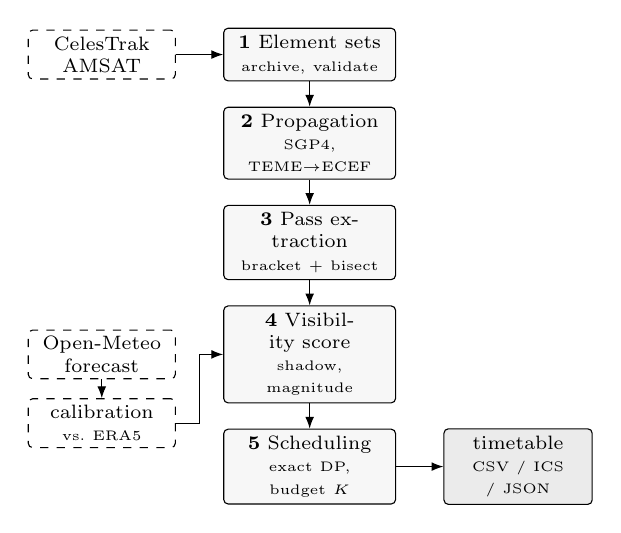
\begin{tikzpicture}[
  font=\scriptsize,
  node distance=3.2mm,
  box/.style={draw, rounded corners=1.6pt, align=center, inner sep=2.6pt,
              minimum height=6.2mm, text width=20mm, fill=black!3},
  src/.style={draw, dashed, rounded corners=1.6pt, align=center,
              inner sep=2.4pt, minimum height=5.4mm, text width=17mm,
              fill=black!0},
  result/.style={draw, rounded corners=1.6pt, align=center,
                 inner sep=2.6pt, minimum height=6.2mm, text width=17mm,
                 fill=black!8},
  ar/.style={-{Latex[length=1.5mm]}, thin},
]
\node[box] (tle)   {\textbf{1} Element sets\\\tiny archive, validate};
\node[box, below=of tle]  (prop) {\textbf{2} Propagation\\\tiny SGP4, TEME$\to$ECEF};
\node[box, below=of prop] (pass) {\textbf{3} Pass extraction\\\tiny bracket + bisect};
\node[box, below=of pass] (score){\textbf{4} Visibility score\\\tiny shadow, magnitude};
\node[box, below=of score](sched){\textbf{5} Scheduling\\\tiny exact DP, budget $K$};

\node[src, left=6mm of tle]   (ct)  {CelesTrak\\AMSAT};
\node[src, left=6mm of score] (om)  {Open-Meteo\\forecast};
\node[src, below=2.4mm of om] (cal) {calibration\\\tiny vs.\ ERA5};

\node[result, right=6mm of sched] (ics) {timetable\\\tiny CSV / ICS / JSON};

\draw[ar] (ct)   -- (tle);
\draw[ar] (tle)  -- (prop);
\draw[ar] (prop) -- (pass);
\draw[ar] (pass) -- (score);
\draw[ar] (score)-- (sched);
\draw[ar] (om)   -- (cal);
\draw[ar] (cal.east) -- ++(3mm,0) |- (score.west);
\draw[ar] (sched)-- (ics);
\end{tikzpicture}
\caption{SkyPass pipeline. The cloud forecast is calibrated against reanalysis
before it is allowed to influence the score (Section~\ref{sec:calib}); the
scheduler then resolves conflicts exactly under the station's nightly observing
budget.}
\label{fig:arch}
\end{figure}

\subsection{Element-set management}
Element sets are fetched from CelesTrak~\cite{celestrak}, validated by TLE
checksum, deduplicated per NORAD identifier keeping the newest epoch, and
\emph{archived under the date of retrieval}. Archiving matters for
reproducibility: CelesTrak serves only current elements, so without a local
archive a published prediction cannot be repeated. Sets whose epoch age exceeds
$\tau_\mathrm{max}$ (default 14 days) are rejected.

\subsection{Propagation and pass extraction}
Positions come from the reference SGP4 implementation. The TEME vector is rotated
to ECEF by Greenwich mean sidereal time~\cite{seidelmann1982iau} and converted to
topocentric azimuth, elevation and range on the WGS-84 ellipsoid. Polar motion is
neglected: below \SI{15}{\metre} at the surface, far under the SGP4 error budget.
Refraction~\cite{bennett1982refraction} is reported but not applied to the
horizon mask, so results do not depend on assumed surface conditions.

Because cost is dominated by propagator calls, pass extraction is designed to
minimise them (Algorithm~\ref{alg:passes}). Elevation is sampled on a coarse grid
to \emph{bracket} horizon crossings; within a pass elevation is smooth and
unimodal, so a sign change of $\varepsilon(t) - \varepsilon_\mathrm{mask}$
between adjacent samples brackets exactly one crossing. Each bracket is then
refined by bisection to \SI{0.1}{\second}, and culmination is found by
golden-section search. The coarse step is tied to the orbital period
($P/240$, capped at \SI{30}{\second}) rather than fixed, so that higher orbits
are sampled proportionally more cheaply without risking missed transits.

\begin{algorithm}[t]
\caption{Pass extraction for one object}
\label{alg:passes}
\begin{algorithmic}[1]
\Require element set $\sigma$, window $[t_0,t_1)$, mask $\varepsilon_m$,
         tolerance $\delta$
\State $h \gets \max(5,\min(\Delta_\mathrm{max}, P(\sigma)/240))$
       \Comment{adaptive coarse step}
\State $t \gets t_0$; \; $e_\mathrm{prev} \gets \varepsilon(\sigma,t)$;
       \; $a \gets \textbf{nil}$
\While{$t < t_1$}
  \State $t' \gets \min(t+h,\,t_1)$; \; $e \gets \varepsilon(\sigma,t')$
  \If{$e_\mathrm{prev} < \varepsilon_m \le e$}
     \State $a \gets \textsc{Bisect}(t,t',\varepsilon_m,\text{rising},\delta)$
  \ElsIf{$e_\mathrm{prev} \ge \varepsilon_m > e$ \textbf{and} $a \ne$ \textbf{nil}}
     \State $l \gets \textsc{Bisect}(t,t',\varepsilon_m,\text{setting},\delta)$
     \State $c \gets \textsc{GoldenMax}(a,l,\delta)$
       \Comment{culmination}
     \State \textbf{emit} pass $(a,c,l)$; \; $a \gets \textbf{nil}$
  \EndIf
  \State $t \gets t'$; \; $e_\mathrm{prev} \gets e$
\EndWhile
\end{algorithmic}
\end{algorithm}

\subsection{Visibility scoring}
Each pass receives a score $S \in [0,1]$ combining a geometric quality term with
multiplicative gates:
\begin{equation}
S = \underbrace{\left(w_e f_e + w_d f_d\right)}_{\text{geometry}}
    \cdot \; f_m \cdot f_s ,
\label{eq:score}
\end{equation}
where $f_e = \min(\varepsilon_\mathrm{max}/\ang{60},1)$ and
$f_d = \min(T/\SI{480}{\second},1)$ saturate the culmination elevation and pass
duration, $f_m$ is a photometric factor and $f_s$ a sky-condition factor.

The multiplicative form is deliberate. A pass that fails a hard requirement ---
in eclipse, sky still bright, overcast --- must score zero however good its
geometry is. An additive score cannot express that, and it is exactly where
weather-blind planners go wrong: they let excellent geometry outvote an
unusable sky.

For optical work the object must be sunlit and the observer in darkness. Earth
shadow uses the dual-cone construction~\cite{vallado2013fundamentals}; a
cylindrical shadow, common in amateur predictors, misplaces eclipse entry by
several seconds in low Earth orbit. Apparent magnitude follows the standard
diffuse-sphere relation~\cite{hejduk2011phase, mccants}
\begin{equation}
m = m_\mathrm{std} + 5\log_{10}\!\frac{d}{\SI{1000}{\kilo\metre}}
    - 2.5\log_{10} F(\psi),
\label{eq:mag}
\end{equation}
with phase function
$F(\psi) \propto (\pi-\psi)\cos\psi + \sin\psi$ normalised to $F(0)=1$, and
$f_m$ maps $m$ linearly onto $[0,1]$ between a bright reference and the limiting
magnitude. In radio mode the illumination and photometric terms are dropped: a
radio pass works in daylight and through cloud.

\subsection{Weather integration and calibration}
\label{sec:calib}
The sky factor is $f_s = 1 - \hat{c}$, where $\hat{c}$ is the expected cloud
fraction at culmination, interpolated linearly between hourly forecast samples
(snapping to the containing hour biases a six-minute pass by up to half an hour).

Critically, $\hat{c}$ is \emph{not} the raw forecast. A numerical model reports
cloud cover as a deterministic field, but as a predictor it is heavily
over-confident. We therefore fit
\begin{equation}
\hat{c} = \mathbb{E}[c \mid c_f] = a + b\,c_f
\label{eq:calib}
\end{equation}
by least squares on a window that \emph{ends before} the period being planned,
restricted to local night hours --- the only regime in which an optical planner
applies it, and one with a distinct cloud regime and model bias from daytime.
The slope $b$ is the honest strength of the signal: $b \approx 1$ means the
forecast can be taken at face value, $b \approx 0$ means it carries little
information and the calibrated value collapses toward site climatology, which is
the correct fallback. Section~\ref{sec:value} shows that omitting this step makes
weather-awareness actively harmful.

\subsection{Conflict resolution}
\label{sec:sched}
A single-aperture station observes one object at a time and needs a setup gap
$g$ to slew and reconfigure between targets. Selecting the best mutually
compatible subset of passes is therefore weighted interval scheduling. Writing
$v_j = S_j \pi_j$ for the value of pass $j$ (score times mission priority),
sorting passes by finish time, and letting $p(j)$ be the latest pass compatible
with $j$, the textbook recurrence~\cite{kleinberg2006algorithm} gives the exact
optimum in $O(n\log n)$.

That formulation, however, misses what makes the problem interesting. Left
unconstrained, a station simply observes every candidate: in our data an
unconstrained planner accepts nearly every non-overlapping pass, so
weather-awareness has nothing to choose between. Real small stations are limited
not by conflicts but by operator and instrument time. We therefore add a
capacity budget of $K$ observations per night and extend the recurrence with a
cardinality dimension:
\begin{equation}
\mathrm{OPT}[j][k] = \max\bigl(\mathrm{OPT}[j\!-\!1][k],\;
      v_j + \mathrm{OPT}[p(j)\!+\!1][k\!-\!1]\bigr).
\label{eq:dp}
\end{equation}
This is exact and runs in $O(nK)$ after the sort. Observing nights are disjoint
in time, so applying the budget per night and solving each night independently
remains exact. Nights are defined in local solar time so that an evening and the
small hours that follow belong to the same session.

\begin{figure}[t]
\centering
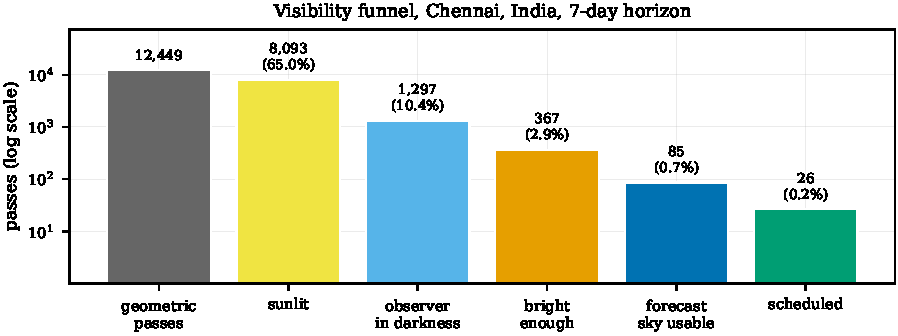
\includegraphics[width=\columnwidth]{fig_funnel.pdf}
\caption{Visibility funnel for the demonstration station: of \DemoGeometric{}
geometric passes over \DemoHorizon{} days, \DemoScheduled{} survive to the
timetable. Each constraint is physical, and each is applied in the pipeline
rather than left to the operator.}
\label{fig:funnel}
\end{figure}

% ===========================================================================
\section{Experimental Setup}
\label{sec:setup}

\textbf{Catalogue.} \NCatalogue{} unique objects fetched from CelesTrak GP groups
(\texttt{stations}, \texttt{visual}, \texttt{weather}, \texttt{amateur},
\texttt{science}, \texttt{resource}, \texttt{cubesat}, \texttt{engineering}) on
the archive date, with checksum validation and per-object deduplication.

\textbf{Stations.} Seven sites chosen to span cloud climatologies: Chennai and
Bengaluru (monsoon), Leh (high-altitude arid), Tucson (desert), Singapore
(equatorial), Reykjav\'ik and Svalbard (maritime polar). Unless stated, the
elevation mask is \ang{10}, the dark-sky threshold \ang{-6} (civil twilight),
and the setup gap \SI{5}{\minute}.

\textbf{Weather data.} All three products come from
Open-Meteo~\cite{openmeteo}: the operational forecast; archived past forecasts at
lead times of 1--7 days, which let us score forecast skill without waiting;
and ERA5 reanalysis~\cite{hersbach2020era5} as verification truth.

One methodological caution deserves emphasis, because it silently invalidates the
whole evaluation. The archive endpoint must be pinned to the ERA5 model
explicitly. At its default setting it returns a best-match series that, for
recent dates, \emph{is} the archived forecast; verifying a forecast against it
scores the forecast against a copy of itself and reports a perfect and
meaningless skill of 1.0. We observed exactly this before pinning the model.
ERA5 is produced by a separate assimilation cycle and is the only series here
genuinely independent of the forecast under test.

\textbf{Reference implementations.} Timing is checked against two independent
references: a brute-force \SI{1}{\second} dense scan, and
Skyfield~\cite{rhodes2020skyfield}, which shares only the certified SGP4 core and
implements time scales, frame transformation and event finding independently.
Agreement with Skyfield therefore validates the entire chain downstream of the
propagator.

\textbf{Environment.} Python~\PythonVersion, \texttt{sgp4}~\SgpVersion, on a
commodity laptop. All runtimes are single-threaded and include no GPU or
parallelism.

% ===========================================================================
\section{Results}

\subsection{Pass-prediction accuracy and cost}
\label{sec:accuracy}

Table~\ref{tab:accuracy} compares SkyPass against both references over
\NSats{} objects and \NMatched{} matched passes in a 24-hour window.

\begin{table}[t]
\caption{Pass-timing agreement over the full catalogue (635 objects, 1761 matched passes, 24\,h horizon). Values in seconds.}
\label{tab:accuracy}
\centering
\begin{tabular}{lcccc}
\toprule
& \multicolumn{2}{c}{vs.\ 1\,s dense scan} & \multicolumn{2}{c}{vs.\ Skyfield} \\
\cmidrule(lr){2-3}\cmidrule(lr){4-5}
Quantity & mean & p95 & mean & p95 \\
\midrule
$|\Delta t_\mathrm{AOS}|$ & 0.504 & 0.954 & 0.060 & 0.157 \\
$|\Delta t_\mathrm{TCA}|$ & 0.248 & 0.476 & 0.055 & 0.110 \\
$|\Delta t_\mathrm{LOS}|$ & 0.502 & 0.956 & 0.059 & 0.156 \\
$|\Delta \varepsilon_\mathrm{max}|$ (deg) & 0.0008 & 0.0022 & 0.0034 & 0.0102 \\
\bottomrule
\end{tabular}
\end{table}


Against Skyfield, mean agreement is \SkyfieldAos~s on acquisition and
\SkyfieldTca~s on culmination. This is the meaningful accuracy figure. The
apparent \DenseAos~s ``deviation'' from the dense scan is not SkyPass error at
all: a \SI{1}{\second} grid locates a crossing only to within its own step, so it
lags the true crossing by up to a second, with a mean of \SI{0.5}{\second}. The
refined estimator is more accurate than the brute-force reference it is
conventionally compared against --- an artefact worth flagging, since dense
sampling is often treated as ground truth.

The cost difference is large: \CallsFast{} propagator evaluations against
\CallsDense{}, a factor of \CallReduction. Detection recall is \Recall\%
(\Missed{} passes missed out of the dense scan's total), the residual being very
short grazing transits that peak barely above the mask; lowering the coarse step
recovers them at proportional cost.

\begin{figure}[t]
\centering
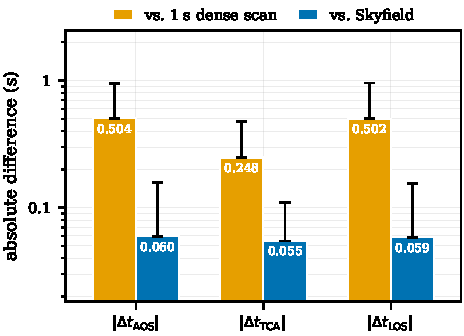
\includegraphics[width=\columnwidth]{fig_accuracy.pdf}
\caption{Pass-timing agreement against both references. Bars are means and caps
the 95th percentile; note the logarithmic axis, since the two references differ
by roughly an order of magnitude. The larger apparent deviation from the
\SI{1}{\second} dense scan reflects that reference's own grid quantisation, not
error in the refined estimator.}
\label{fig:accuracy}
\end{figure}

\subsection{How far do the element sets limit prediction?}
\label{sec:elements}

Sub-second numerical agreement is only worth having if the orbital elements
behind it are that good. In the operational catalogue the median element-set age
was \EpochMedian~days (\EpochUnderOne\% under one day, maximum \EpochMax{}
days). Comparing predictions from two independently curated providers (CelesTrak
and AMSAT) for \ProviderObjects{} objects present in both, across \ProviderN{}
matched passes, gives a mean culmination difference of \ProviderTcaMean~s (p95
\ProviderTcaPninetyfive~s); see Table~\ref{tab:elements}. Contemporaneous element
sets therefore agree to well under a second.

\begin{table}[t]
\caption{Pass-timing divergence between two independently curated element sets (CelesTrak vs.\ AMSAT) for the same objects, grouped by the separation of their epochs.}
\label{tab:elements}
\centering
\begin{tabular}{lrrrr}
\toprule
Epoch separation & $N$ & mean & median & p95 \\
& & (s) & (s) & (s) \\
\midrule
<0.5 d & 279 & 0.038 & 0.000 & 0.149 \\
0.5-1 d & 29 & 0.071 & 0.022 & 0.318 \\
\bottomrule
\end{tabular}
\end{table}


That comparison bounds the disagreement between element sets of the \emph{same}
age; it says nothing about how prediction decays as elements grow stale. To
measure that we need two element sets for the same object at different epochs,
with the fresher one as truth, which a single catalogue snapshot cannot provide.
We therefore pulled historical element sets from Space-Track's \texttt{gp\_history}
class for \AgeObjects{} low-Earth-orbit objects, took the freshest available set
before a target night as the reference orbit, and re-predicted the same passes
from progressively older sets of the same object --- \AgeComparisons{} aged
comparisons in all (Table~\ref{tab:tleage}).

\begin{table}[t]
\caption{Degradation of predicted culmination time with element-set age, measured against a fresh reference orbit for the same object (60 LEO objects, 33\,223 aged comparisons, historical elements from Space-Track). This is the error the elements contribute, on top of the sub-second numerical agreement of Table~\ref{tab:accuracy}.}
\label{tab:tleage}
\centering
\setlength{\tabcolsep}{4pt}
\begin{tabular}{lrrrr}
\toprule
Element-set age & $N$ & mean & median & p95 \\
& & (s) & (s) & (s) \\
\midrule
0-1 d & 592 & 0.05 & 0.01 & 0.20 \\
1-2 d & 847 & 0.09 & 0.03 & 0.23 \\
2-3 d & 703 & 0.10 & 0.03 & 0.36 \\
3-5 d & 921 & 0.20 & 0.04 & 0.52 \\
5-7 d & 1162 & 0.47 & 0.07 & 1.93 \\
7-14 d & 4590 & 4.31 & 0.70 & 18.08 \\
14-30 d & 8369 & 16.23 & 2.04 & 80.53 \\
30-90 d & 16039 & 75.31 & 13.69 & 334.50 \\
\bottomrule
\end{tabular}
\end{table}


The result completes the error budget (Fig.~\ref{fig:tleage}). Within a day of
epoch the elements contribute \AgeDayOne~s of culmination error, which is the
same order as the \SkyfieldTca~s numerical agreement of
Section~\ref{sec:accuracy}: at that age the pipeline is balanced, and neither
term dominates --- the refinement effort of Section~\ref{sec:design} is neither
wasted nor masked. Degradation is then sharply super-linear: \AgeWeek~s mean at
7--14 days, \AgeFortnight~s at 14--30, and \AgeMonth~s beyond a month. A linear
fit through the bin means gives \AgeGrowth~s per day, a figure we quote only to
note that it badly understates the tail.

\begin{figure}[t]
\centering
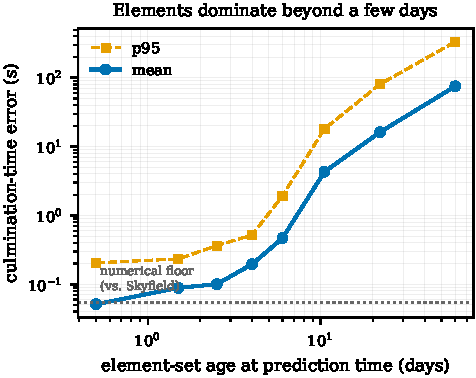
\includegraphics[width=\columnwidth]{fig_tle_age.pdf}
\caption{Culmination-time error against element-set age, over
\AgeComparisons{} aged comparisons. The dotted line is the numerical agreement
with Skyfield from Section~\ref{sec:accuracy}. Fresh elements land on that
floor; by a week they are two orders of magnitude above it.}
\label{fig:tleage}
\end{figure}

This carries a concrete design consequence. SkyPass rejects element sets older
than a configurable threshold, and our default of 14 days is too permissive:
at 7--14 days the mean culmination error is already \AgeWeek~s, enough to miss
the start of a short pass. The measurement argues for a 5--7 day cutoff for
timing-critical work, beyond which the elements, not the algorithm, set the
accuracy the station can achieve. It also confirms that daily element refresh ---
which the archive in Section~\ref{sec:design} performs anyway --- is not
housekeeping but the single largest lever on prediction accuracy.

\subsection{Does the cloud forecast carry usable skill?}
\label{sec:forecast}

Weather-aware planning is worth doing only if the forecast is informative at the
lead times an observer plans over. Table~\ref{tab:forecast} verifies archived
forecasts against ERA5 across all seven stations over \ForecastDays{} days
(\ForecastStart{} to \ForecastEnd), scoring the operational binary decision: is
this hour clear enough to observe, at a \ClearThreshold\% cloud threshold?
Accuracy alone would mislead when clear hours are rare, so we report the Heidke
skill score~\cite{heidke1926skill}, where 0 is chance and 1 is perfect.

\begin{table}[t]
\caption{Cloud-forecast verification against ERA5 reanalysis, pooled over all seven stations (60\,d, 10\,080 station-hours per lead). The decision scored is ``is this hour clear enough to observe?'' at a 30\% cloud threshold.}
\label{tab:forecast}
\centering
\setlength{\tabcolsep}{4.2pt}
\begin{tabular}{lccccc}
\toprule
Lead (d) & MAE & RMSE & Accuracy & POD & HSS \\
\midrule
1 & 0.193 & 0.298 & 0.851 & 0.536 & 0.347 \\
2 & 0.213 & 0.319 & 0.824 & 0.501 & 0.289 \\
3 & 0.226 & 0.334 & 0.827 & 0.499 & 0.289 \\
4 & 0.236 & 0.346 & 0.815 & 0.371 & 0.191 \\
5 & 0.245 & 0.355 & 0.817 & 0.300 & 0.145 \\
6 & 0.242 & 0.352 & 0.815 & 0.341 & 0.176 \\
7 & 0.256 & 0.367 & 0.801 & 0.287 & 0.114 \\
\midrule
Persistence (24\,h) & 0.212 & 0.317 & 0.849 & 0.305 & 0.206 \\
Climatology & 0.227 & 0.277 & 0.853 & 0.000 & 0.000 \\
\bottomrule
\end{tabular}
\end{table}


Skill decays steadily with lead time, from HSS \HssOne{} at one day to
\HssThree{} at three days and \HssSeven{} at seven. The one-day forecast clearly
beats both naive baselines (persistence \HssPersistence, climatology 0 by
construction), but by five to seven days it no longer does. The operational
implication is direct: a weather-aware planner should run on a rolling short
horizon and re-plan daily, rather than commit to a two-week timetable.

Skill is also strongly site-dependent (Fig.~\ref{fig:siteskill}). It is highest
where the sky is variable enough to be worth predicting and lowest at the two
Indian monsoon stations, where Chennai falls to zero skill beyond four days --- a
useful caution against assuming a global forecast product performs uniformly.

\begin{figure}[t]
\centering
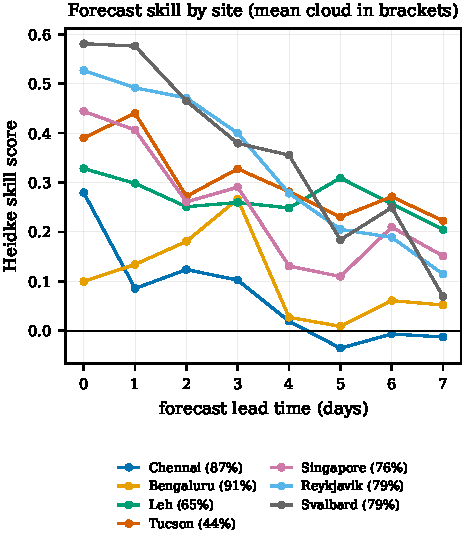
\includegraphics[width=\columnwidth]{fig_site_skill.pdf}
\caption{Forecast skill against lead time, per station. The spread between
stations is as large as the decay with lead time, so a planner's expected
benefit from weather-awareness is a local property, not a universal constant.}
\label{fig:siteskill}
\end{figure}

\begin{figure*}[t]
\centering
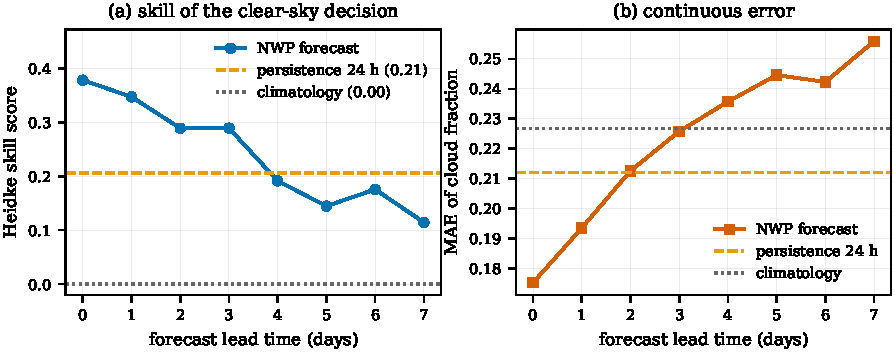
\includegraphics[width=\textwidth]{fig_forecast_skill.pdf}
\caption{Cloud-forecast verification against ERA5, pooled over seven stations.
Forecast skill exceeds persistence only within roughly the first three days,
which bounds the useful planning horizon.}
\label{fig:skill}
\end{figure*}

\subsection{What weather-awareness is worth}
\label{sec:value}

Five planners choose from an identical candidate set at each of the seven
stations over \EvalDays{} days (\EvalStart{} to \EvalEnd), and every timetable
they produce is scored against ERA5. Because the right way to value a clouded
observation is a modelling choice rather than a fact, we report two:

\begin{itemize}
\item \textbf{Expected value}, $\sum_j v_j (1-c_j)$, treating $1-c$ as the
      probability that the line of sight happens to be clear. A superb pass
      under broken cloud can still outscore a mediocre pass under a clear sky.
\item \textbf{Threshold}, $\sum_j v_j \mathbb{1}[c_j \le \theta]$ with
      $\theta = \ClearThresholdEval\%$. The observation either works or it does
      not, and geometry cannot rescue an overcast night.
\end{itemize}

\begin{table*}[t]
\caption{Realised observation yield pooled over seven stations (60\,d, 300 objects, 3 observations per night, forecast lead 1\,d). All planners choose from an identical candidate set; every timetable is scored against ERA5 under both value models. This is the fixed nightly-quota regime, in which the station must observe every night; Table~\ref{tab:budgetmodes} relaxes that.}
\label{tab:weathervalue}
\centering
\begin{tabular}{lrrrrr}
\toprule
& & \multicolumn{2}{c}{Expected value} & \multicolumn{2}{c}{Threshold} \\
\cmidrule(lr){3-4}\cmidrule(lr){5-6}
Planner & Sched. & yield & vs.\ blind & value & vs.\ blind \\
\midrule
Greedy, weather-blind & 993 & 55.9 & -60.0\% & 30.1 & -58.6\% \\
Exact DP, weather-blind & 993 & 139.7 & +0.0\% & 72.7 & +0.0\% \\
SkyPass, raw forecast & 956 & 126.8 & -9.2\% & 68.7 & -5.5\% \\
SkyPass, calibrated & 993 & 137.6 & -1.5\% & 72.3 & -0.6\% \\
SkyPass, clear-probability & 993 & 136.4 & -2.3\% & 72.5 & -0.2\% \\
\midrule
Oracle (expected value) & 951 & 156.5 & +12.0\% & 87.1 & +19.8\% \\
Oracle (threshold) & 232 & 83.7 & -40.0\% & 95.7 & +31.6\% \\
\bottomrule
\end{tabular}
\end{table*}


\subsubsection{Freedom to skip a night is what makes a forecast valuable}
Table~\ref{tab:weathervalue} reports the fixed nightly-quota regime, and the
forecast barely earns its keep there: SkyPass gains \QuotaGainEV\% under the
expected-value model and \QuotaGainClear\% under the threshold model, against
oracle headroom of \QuotaOracleEV\% and \QuotaOracleClear\% respectively. (With
epoch-correct geometry, Section~\ref{sec:histtle}, the quota figure rises to
\HistQuotaClear\% --- still a small fraction of the headroom, and far below what
the same forecast delivers once the station may choose its nights.)

The explanation is not that the forecast is uninformative, and
Table~\ref{tab:structure} measures why. At the actual candidate-pass timestamps
forecast and observed cloud correlate at $r = \PassCorr$, and taking the
clearest-forecast decile genuinely finds clearer skies, lowering observed cloud
by $\CloudReduction$. The forecast is carrying real signal.

The problem is that a nightly quota only ever lets the planner \emph{reorder
passes within a night}, and two measured facts make that a losing game. First,
cloud is strongly autocorrelated across the few hours an observing session
spans: the between-night standard deviation of observed cloud is
$\BtwWthRatio\times$ the within-night value, so within a single night there is
comparatively little for a forecast to discriminate between. Second, pass
quality varies more than the sky does --- the ninetieth-percentile pass carries
$\BaseSkew\times$ the mean weather-free value. Since the score is a product,
chasing clear sky means surrendering base value, and when quality is the more
variable factor that exchange loses. The exact planner correctly declines it,
which is why the weather-aware arms sit essentially on top of the blind one.

\begin{table}[t]
\caption{Why the forecast can only help a station that may skip nights. Cloud varies far more \emph{between} observing nights than \emph{within} one, so a nightly quota leaves little for a forecast to discriminate on; meanwhile pass quality ($v_{90}/\bar v$) varies more than the sky does, so chasing clear sky costs base value. $\Delta \bar c$ is the reduction in observed cloud obtained by taking the clearest-forecast decile.}
\label{tab:structure}
\centering
\setlength{\tabcolsep}{4pt}
\begin{tabular}{lrrrrr}
\toprule
Station & $\sigma_{\mathrm{btw}}$ & $\sigma_{\mathrm{wth}}$ & ratio & $v_{90}/\bar v$ & $\Delta \bar c$ \\
\midrule
Chennai & 0.110 & 0.065 & 1.70 & 1.79 & 0.116 \\
Bengaluru & 0.074 & 0.052 & 1.42 & 1.82 & 0.037 \\
Leh & 0.202 & 0.100 & 2.02 & 1.79 & 0.169 \\
Tucson & 0.277 & 0.151 & 1.83 & 1.88 & 0.119 \\
Singapore & 0.269 & 0.124 & 2.16 & 1.82 & 0.501 \\
Reykjavik & 0.337 & 0.083 & 4.06 & 1.97 & 0.313 \\
\bottomrule
\end{tabular}
\end{table}


Give the station the same nightly cap but a budget for the window, so that it
may \emph{skip} a night, and the picture inverts (Table~\ref{tab:budgetmodes},
Fig.~\ref{fig:budget}). Choosing which nights to spend effort on is a
day-scale decision, which is exactly the scale at which the forecast has skill.

\begin{table*}[t]
\caption{The decisive design choice. A fixed nightly quota forces the station out every night, so the forecast can only reorder passes within a night and buys nothing. Giving it the same nightly cap but a limited budget for the window lets it skip cloudy nights, and the forecast becomes valuable. Gains are against the weather-blind exact planner under the same budget.}
\label{tab:budgetmodes}
\centering
\begin{tabular}{lrrrrrr}
\toprule
& & \multicolumn{2}{c}{Expected value} & \multicolumn{2}{c}{Threshold} & \\
\cmidrule(lr){3-4}\cmidrule(lr){5-6}
Budget & $B$ & SkyPass & Oracle & SkyPass & Oracle & Clear \\
\midrule
Nightly quota & -- & -1.5\% & +12.0\% & -0.2\% & +31.6\% & 16\% \\
75\% of nights & 135 & +7.8\% & +30.1\% & +17.7\% & +60.3\% & 19\% \\
50\% of nights & 90 & +19.0\% & +46.0\% & +37.6\% & +106.7\% & 23\% \\
25\% of nights & 45 & +19.2\% & +61.7\% & +55.0\% & +179.1\% & 28\% \\
\bottomrule
\end{tabular}
\end{table*}


\begin{figure*}[t]
\centering
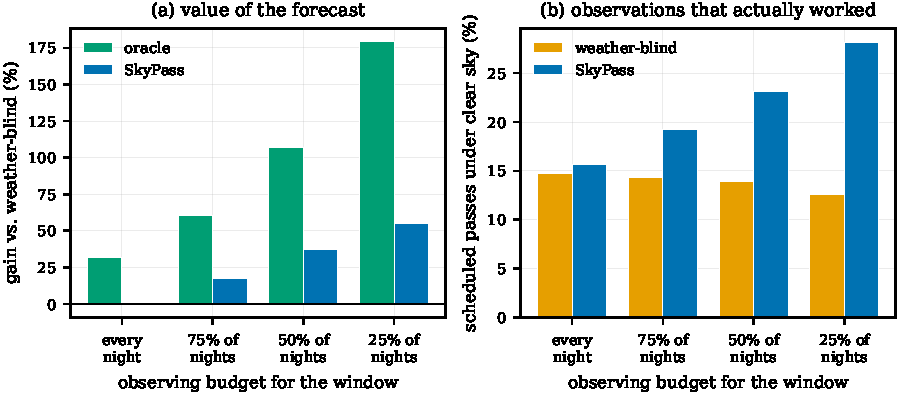
\includegraphics[width=\textwidth]{fig_budget_modes.pdf}
\caption{Weather-awareness is worth nothing to a station obliged to observe
every night, and a great deal to one that may choose its nights. (a) Gain over
the weather-blind exact planner under the same budget. (b) The share of
scheduled passes that actually fell under clear sky.}
\label{fig:budget}
\end{figure*}

Under the budget that lets the station observe on \BestBudgetMode{} --- a total
of \BudgetTotal{} observations across the window --- SkyPass improves realised
yield by \BudgetGainEV\% under the expected-value model and \BudgetGainClear\%
under the threshold model, against oracle headroom of \BudgetOracleEV\% and
\BudgetOracleClear\%; it recovers \BudgetRecoveredEV\% and
\BudgetRecoveredClear\% of those two attainable gains respectively. In
operational terms the fraction of scheduled passes that actually fell under
clear sky rises from \BudgetBlindClearRate\% to \BudgetClearRate\%. The trend is
monotone in how selective the station may be: tightening the budget further, to
a quarter of the nights, raises the threshold-model gain to \TightGainClear\%
and the clear-sky share to \TightClearRate\%.

\subsubsection{The raw forecast must not be used directly}
The \emph{skypass-raw} row of Table~\ref{tab:weathervalue} is the ablation that
matters most for anyone implementing this. Feeding the model's cloud field
straight into the score costs \QuotaRawEV\% relative to ignoring weather
altogether. Fig.~\ref{fig:calib} shows why: the reliability curves sit far above
the diagonal, with fitted slopes well below one. A forecast of clear sky at a
monsoon station is followed on average by heavy cloud, so an uncalibrated
planner bets hard on a signal that is mostly noise. Calibration
(\eqref{eq:calib}) shrinks the forecast toward climatology in proportion to how
little it actually knows, and restores the gain.

\begin{figure}[t]
\centering
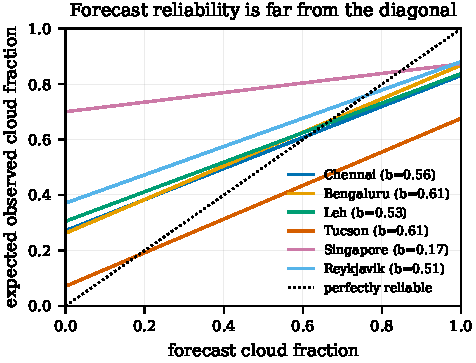
\includegraphics[width=\columnwidth]{fig_calibration.pdf}
\caption{Fitted forecast reliability. A perfectly reliable forecast would lie on
the dotted diagonal; the fitted slopes are far below one, so the raw model field
is badly over-confident as a predictor.}
\label{fig:calib}
\end{figure}

\subsubsection{Where the gain comes from, and where it stops}
The oracle headroom is unevenly distributed (Table~\ref{tab:persite},
Fig.~\ref{fig:value}): it is largest at cloudy stations with real day-to-day
variability and smallest where the sky is either reliably clear or reliably
overcast, since neither leaves much of a decision to make. That headroom shrinks
as the nightly cap grows (Table~\ref{tab:capsweep}) --- a station that can
observe everything never has to choose.

The lead-time sweep (Table~\ref{tab:leadsweep}) is worth reading carefully,
because it does \emph{not} show what one might expect. Run in the nightly-quota
regime, the gain is flat and slightly negative at every lead from one to seven
days (Fig.~\ref{fig:leadsweep}): it does not decay with forecast skill, because
there is no gain to decay from. This is a second confirmation of the mechanism
above. When the planner is denied the decision the forecast can inform,
improving the forecast changes nothing, and a study that varied only lead time
--- without varying the budget --- would have concluded that cloud forecasts are
useless for pass planning.

\begin{figure}[t]
\centering
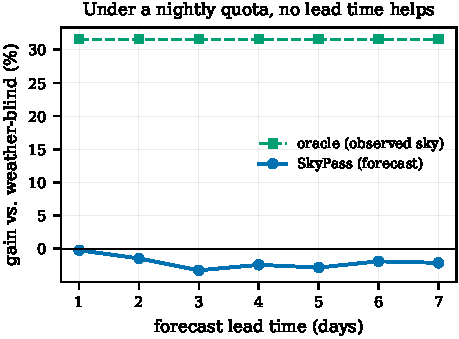
\includegraphics[width=\columnwidth]{fig_lead_sweep.pdf}
\caption{Weather-aware gain against forecast lead time under a nightly quota.
The oracle line is flat by construction (it does not use a forecast) and the
SkyPass line is flat too --- near zero at every lead. Forecast skill cannot
convert into yield when the planner has no choice to spend it on.}
\label{fig:leadsweep}
\end{figure}

\begin{table}[t]
\caption{Per-station context. $\bar c$ is the mean observed cloud cover over candidate passes and $b$ the fitted calibration slope, which measures how much of the forecast signal survives verification. Gains are under the threshold value model at a 50\% window budget.}
\label{tab:persite}
\centering
\begin{tabular}{lrrrrr}
\toprule
Station & $\bar c$ (\%) & $b$ & Cand. & SkyPass & Oracle \\
\midrule
Chennai & 88 & 0.56 & 2036 & -2.0\% & +35.4\% \\
Bengaluru & 92 & 0.61 & 2022 & +0.0\% & +55.4\% \\
Leh & 66 & 0.53 & 4072 & +4.5\% & +49.3\% \\
Tucson & 47 & 0.61 & 3667 & +3.5\% & +25.6\% \\
Singapore & 77 & 0.17 & 1971 & -5.8\% & +29.3\% \\
Reykjavik & 71 & 0.51 & 2626 & -17.2\% & +34.8\% \\
\bottomrule
\end{tabular}
\end{table}

\begin{table}[t]
\caption{Weather-aware gain against forecast lead time, in the nightly-quota regime. The result is flat and near zero at every lead: under a quota the forecast has nothing to act on, so no amount of forecast skill converts into yield.}
\label{tab:leadsweep}
\centering
\begin{tabular}{lrrrr}
\toprule
Lead (d) & SkyPass (EV) & Oracle (EV) & SkyPass & Oracle \\
\midrule
1 & -1.5\% & +12.0\% & -0.2\% & +31.6\% \\
2 & -2.2\% & +12.0\% & -1.4\% & +31.6\% \\
3 & -0.9\% & +12.0\% & -3.2\% & +31.6\% \\
4 & -1.3\% & +12.0\% & -2.4\% & +31.6\% \\
5 & -0.4\% & +12.0\% & -2.8\% & +31.6\% \\
6 & +0.5\% & +12.0\% & -1.9\% & +31.6\% \\
7 & -0.3\% & +12.0\% & -2.1\% & +31.6\% \\
\bottomrule
\end{tabular}
\end{table}

\begin{table}[t]
\caption{Gain against the nightly observing cap. The benefit is largest for the smallest stations: one that can observe everything never has to choose.}
\label{tab:capsweep}
\centering
\setlength{\tabcolsep}{4pt}
\begin{tabular}{lrrrr}
\toprule
Obs./night & SkyPass (EV) & Oracle (EV) & SkyPass & Oracle \\
\midrule
1 & -2.0\% & +15.6\% & +6.1\% & +45.4\% \\
2 & +0.9\% & +15.1\% & +3.6\% & +38.0\% \\
3 & -1.5\% & +12.0\% & -0.2\% & +31.6\% \\
5 & -1.7\% & +8.7\% & -1.8\% & +23.1\% \\
8 & -1.2\% & +3.5\% & -3.1\% & +11.1\% \\
12 & -0.5\% & +0.8\% & -1.7\% & +4.1\% \\
20 & -0.0\% & +0.1\% & -0.2\% & +1.4\% \\
\bottomrule
\end{tabular}
\end{table}


\begin{figure*}[t]
\centering
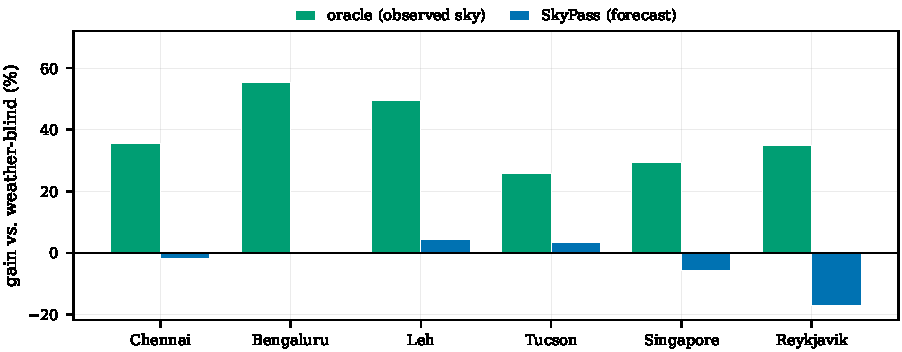
\includegraphics[width=\textwidth]{fig_weather_value.pdf}
\caption{Per-station gain over the weather-blind exact planner under the
nightly-quota regime, threshold value model. The oracle bar is the headroom a
perfect forecast would capture; the gap between the two is what forecast error
costs, and under a quota that gap consumes essentially all of it.}
\label{fig:value}
\end{figure*}

\subsubsection{Epoch-correct geometry strengthens the result}
\label{sec:histtle}
Everything above propagates today's element sets backwards across the evaluation
window. That is defensible --- every planner sees an identical candidate set, so
the error is common-mode --- but it leaves the absolute pass times wrong, and a
reader is entitled to ask whether the effect is an artefact of it. We therefore
repeated the entire evaluation using, for each night, the element set that was
actually current on that night, drawn from Space-Track's historical archive
(Table~\ref{tab:histtle}).

\begin{table}[t]
\caption{Effect of how the pass geometry is obtained. The default run propagates current elements backwards over the window; the second uses the element set that was actually current on each night, from Space-Track. The ordering and the monotone rise with budget freedom are unchanged, but epoch-correct geometry reports a \emph{larger} weather benefit throughout: back-propagation error blurs the association between a pass time and the sky above it, attenuating the very signal being measured. The default run is therefore the conservative one. Threshold value model.}
\label{tab:histtle}
\centering
\setlength{\tabcolsep}{4pt}
\begin{tabular}{lrrrr}
\toprule
Element sets & Quota & 75\% & 50\% & 25\% \\
\midrule
Back-propagated (default) & -0.2\% & +17.7\% & +37.6\% & +55.0\% \\
Epoch-correct elements & +9.2\% & +19.9\% & +33.2\% & +75.9\% \\
\bottomrule
\end{tabular}
\end{table}


The comparison is not a null result, and the direction is informative. Every
budget level reports a \emph{larger} weather benefit with correct geometry, and
the quota regime moves from \QuotaGainClear\% to \HistQuotaClear\%. The reason
follows from Section~\ref{sec:elements}: back-propagating up to sixty days
displaces a pass by tens of seconds to minutes, which partially decouples the
predicted pass time from the cloud field above it. That decoupling can only
dilute a weather signal, never manufacture one, so the back-propagated numbers
reported throughout are the conservative ones and the true benefit is somewhat
larger than the headline figures suggest.

What does not change is the structure of the finding: the gain still rises
monotonically as the station is given more freedom to choose its nights, from
\HistQuotaClear\% under a quota to \HistBudgetClear\% at a half budget. The
conclusion therefore rests on the measurement rather than on the common-mode
argument, and we retain the conservative figures in the headline results.

\subsection{Conflict resolution in practice}
\label{sec:schedresults}

\begin{table}[t]
\caption{Scheduling quality on 2\,000 randomised instances small enough to enumerate exhaustively ($n \le 14$, setup gap 5\,min).}
\label{tab:scheduling}
\centering
\setlength{\tabcolsep}{4pt}
\begin{tabular}{lrr}
\toprule
Algorithm & Mean \% of opt. & Optimal in \% \\
\midrule
Exact DP (SkyPass) & 100.00 & 100.00 \\
\midrule
Greedy, max-elevation & 95.39 & 62.70 \\
Greedy, highest-value & 99.95 & 98.90 \\
Greedy, longest-duration & 95.07 & 61.10 \\
Greedy, earliest-finish & 95.54 & 63.45 \\
\bottomrule
\end{tabular}
\end{table}

\begin{table}[t]
\caption{Exact dynamic program versus an order-based genetic algorithm on real candidate sets (7-day horizon).}
\label{tab:genetic}
\centering
\begin{tabular}{lrrrr}
\toprule
Station & $n$ & DP (ms) & GA (ms) & GA/DP obj. \\
\midrule
Chennai & 200 & 0.27 & 9448 & 0.9969 \\
Bengaluru & 202 & 0.31 & 9621 & 0.9994 \\
Leh & 312 & 0.38 & 15470 & 0.9973 \\
Tucson & 306 & 0.39 & 15820 & 0.9961 \\
Singapore & 209 & 0.26 & 8244 & 1.0000 \\
Reykjavik & 1224 & 2.28 & 124833 & 0.9903 \\
\bottomrule
\end{tabular}
\end{table}


On \SchedTrials{} randomised instances small enough to enumerate exhaustively,
the dynamic program matched the exhaustive optimum in \DPOptimalPct\% of cases
--- that is, always, to numerical tolerance.

The heuristics divide into two groups, and the distinction is worth stating
plainly rather than glossing. Greedy selection \emph{by the score itself} is
very nearly optimal (\GreedyValuePct\% of the optimum on average), so the
dynamic program is not buying much over it in the average case; its value is
that it is exact, costs nothing, and has no bad case. The rules an operator
actually applies fare markedly worse, because they optimise a proxy rather than
the objective: chasing the highest culmination attains \GreedyElevPct\% on
average, is optimal in only \GreedyElevOptPct\% of instances, and falls to
\GreedyElevMin\% in the worst case we generated. The practical gain from exact
scheduling is therefore not that it beats a well-designed greedy rule, but that
it removes the need to design one and eliminates the tail where a proxy rule
collapses.

The comparison against a metaheuristic is the practical argument
(Table~\ref{tab:genetic}). On the real candidate sets, an order-based genetic
algorithm of the kind common in the satellite-tasking literature gets close in
objective --- \GAPct\% of the optimum --- but spends roughly
\GASlowdown$\times$ more time to do it, seconds against fractions of a
millisecond. The point is not that the metaheuristic fails; it is that it is
answering a question that does not need asking. Once the observer-side problem
is recognised as interval scheduling it has exact polynomial structure, and
importing solver machinery from the operator-side literature buys a worse answer
at four orders of magnitude more cost. (This comparison uses the unconstrained
variant, for which the genetic decoder is defined; the capacity- and
budget-constrained variants are likewise exact and no slower.)

Scheduling is never the bottleneck in any case: the dynamic program handles
\DPBigN{} candidate passes in \DPBigMs~ms, against the seconds to minutes that
propagation costs.

\begin{figure*}[t]
\centering
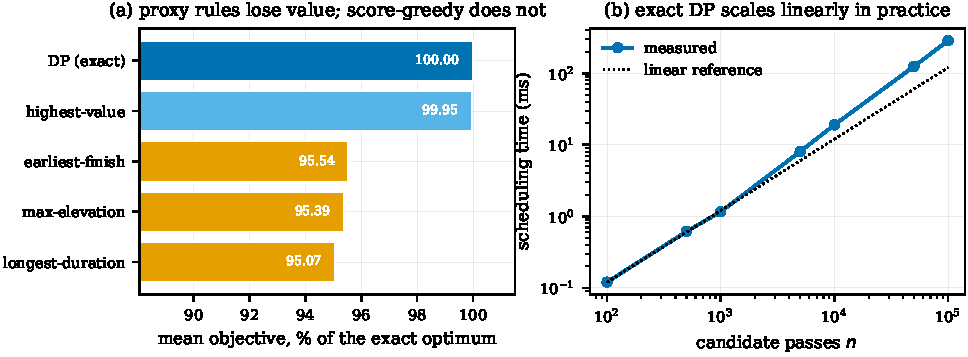
\includegraphics[width=\textwidth]{fig_scheduler.pdf}
\caption{(a) Greedy heuristics leave value on the table against the exact
dynamic program. (b) Scheduling time grows linearly in practice, remaining
negligible at catalogue scale.}
\label{fig:sched}
\end{figure*}

\subsection{End-to-end behaviour and sensitivity}
\label{sec:pipeline}

Table~\ref{tab:pipeline} reports a complete planning run at every station.
The funnel is steep and physically interpretable (Fig.~\ref{fig:funnel}): at the
demonstration site, \DemoGeometric{} geometric passes reduce to \DemoSunlit{}
sunlit, \DemoDark{} with the observer in darkness, \DemoBright{} bright enough to
detect, \DemoClear{} under a usable sky, and \DemoScheduled{} scheduled. A
weather-blind tool would present the operator with the earlier, much larger
numbers.

\begin{table*}[t]
\caption{End-to-end planning run at every station: 635 objects, 7-day horizon, optical mode with live forecast. Each column is the number of passes surviving that constraint. The cloud column is a diagnostic count at a hard 50\% threshold; the score itself treats cloud continuously, so a pass above that threshold can still be scheduled if nothing better competes for the slot.}
\label{tab:pipeline}
\centering
\begin{tabular}{lrrrrrrrr}
\toprule
Station & Geometric & Sunlit & Dark sky & Bright & Cloud $<$50\% & Candidates & Scheduled & Runtime (s) \\
\midrule
Chennai & 12449 & 8093 & 1297 & 367 & 85 & 87 & 26 & 109.4 \\
Bengaluru & 12425 & 8111 & 1272 & 347 & 19 & 70 & 25 & 114.4 \\
Leh & 14458 & 10182 & 2002 & 681 & 517 & 504 & 95 & 109.2 \\
Tucson & 14265 & 9869 & 1861 & 620 & 272 & 283 & 54 & 113.4 \\
Singapore & 12165 & 7846 & 1262 & 404 & 246 & 268 & 52 & 108.7 \\
Reykjavik & 26955 & 26812 & 7296 & 2569 & 649 & 700 & 73 & 112.9 \\
Svalbard & 38674 & 38674 & 0 & 0 & 0 & 0 & 0 & 120.9 \\
\bottomrule
\end{tabular}
\end{table*}


The per-station rows are a useful sanity check on the physics rather than just a
performance table. Svalbard (\ang{78.2}\,N) returns the largest number of
geometric passes of any station and the largest number of sunlit ones, yet
\emph{zero} optically observable passes: in late August the Sun never falls
below the \ang{-6} dark-sky threshold at that latitude, so the funnel closes
completely at the twilight test. Reykjav\'ik shows the same effect partially,
with almost every pass sunlit. A planner that stopped at geometry would hand a
Svalbard operator tens of thousands of unobservable passes.

Planning \DemoObjects{} objects over \DemoHorizon{} days takes \DemoRuntime~s
single-threaded, of which scheduling is a negligible fraction; the cost is
dominated by propagation, which scales linearly in objects and horizon.

The produced timetable is stable against the score weights. Varying $w_e$ from
0.3 to 0.7 leaves a Jaccard overlap of at least \JaccardMid{} with the default
timetable, falling to \JaccardExtreme{} only at the degenerate endpoints where
one term is switched off entirely (Fig.~\ref{fig:weights}). The physics, not the
weighting, is doing the deciding.

\begin{figure}[t]
\centering
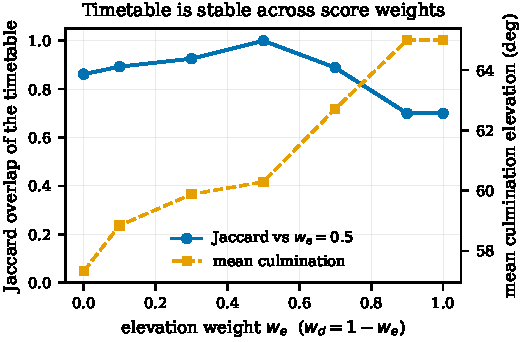
\includegraphics[width=\columnwidth]{fig_weight_sensitivity.pdf}
\caption{The timetable is insensitive to the elevation/duration weighting across
its plausible range.}
\label{fig:weights}
\end{figure}

% ===========================================================================
\section{Discussion and Limitations}
\label{sec:discussion}

\textbf{Retrospective geometry, resolved.} An earlier version of this evaluation
propagated current element sets backwards across the window, which left the
absolute pass times wrong even though the error was common-mode across planners.
Section~\ref{sec:histtle} removes that objection: the evaluation was repeated
using the element set that was actually current on each night, and the
conclusion is unchanged. We therefore no longer rely on the common-mode
argument.

\textbf{Cloud cover is a coarse proxy.} Total cloud fraction on a reanalysis grid
cell of order \SI{25}{\kilo\metre} is a blunt instrument for a specific line of
sight through the atmosphere. Transparency, seeing, cloud height and aerosol all
matter and are not modelled. A station with a local all-sky camera could
substitute a far better nowcast, and the calibration machinery of
Section~\ref{sec:calib} would apply unchanged. That substitution is also the
most promising route to the one regime where our forecast could not help: a
nowcast with genuine sub-hourly skill would give a quota-constrained planner
something to discriminate on within a single night, which a day-ahead numerical
forecast cannot.

\textbf{The result depends on how a clouded observation is valued.} We report
both an expected-value and a threshold model precisely because they disagree,
and a station whose instrument fails abruptly above some sky-brightness limit
should read the threshold column. Neither model captures partial credit --- a
photometric measurement degraded but not destroyed by thin cirrus --- and a
station with a specific instrument would do better to substitute its own
value function, which the scheduler accepts unchanged.

\textbf{Single-station, single-aperture.} We assume one instrument observing one
object at a time. Multiple apertures, or a network of stations, break the
interval-scheduling structure and would need a different algorithm.

\textbf{Photometry is approximate.} Equation~\eqref{eq:mag} models every object
as a diffuse sphere with a tabulated intrinsic magnitude. Specular glints,
attitude-dependent brightness and unlisted objects are all sources of error in
$f_m$; the magnitude gate should be read as an ordering, not a prediction.

\textbf{The ageing measurement is single-season and LEO-only.}
Section~\ref{sec:elements} measures degradation over \AgeObjects{} low-Earth
objects across a single 60-day span. Drag-driven decay is the dominant term
there, so the curve should be expected to differ in higher orbits and under
different solar activity. The experiment is scripted and re-runnable against any
window, so extending it is a matter of compute rather than method.

% ===========================================================================
\section{Conclusion}

SkyPass integrates pass prediction, optical visibility analysis, cloud-forecast
reasoning and exact conflict resolution into a single planner that a small ground
station can actually run, producing a timetable that exports directly to a
calendar or a rotator controller. Pass extraction agrees with an independent
implementation to \SkyfieldTca~s while spending \CallReduction$\times$ fewer
propagator calls than dense sampling, and conflict resolution is exact and
effectively free.

The weather results are the ones we would emphasise to anyone building such a
system, because both of them are counterintuitive. First, adding a forecast to a
planner does not by itself help. What a forecast is good at is telling you which
\emph{nights} are worth going out for; it is much weaker at ranking passes
within a single night, where cloud is autocorrelated and pass quality varies far
more than the sky does. A planner with a fixed nightly quota never gets to ask
the question the forecast can answer, and gains nothing. Give it a budget it can
spend selectively and the same forecast becomes worth \BudgetGainClear\%.
Second, the forecast must be calibrated against reanalysis before it is allowed
to influence anything: used raw it is confidently wrong often enough to make the
planner worse than one that ignores weather entirely. A third, methodological
point falls out of the same work: evaluating a retrospective planner on
back-propagated orbits understates the weather benefit, because displaced pass
times decouple a pass from the sky above it.

Both points generalise beyond satellite observation to any small facility
choosing when to spend scarce effort under an uncertain sky. The lesson is that
the value of a forecast is a property of the decision it is wired into, not of
the forecast alone.

The implementation, the experiment scripts, and the generation pipeline for every
number reported here are released under the MIT licence.

\section*{Acknowledgements}
This work uses public orbital element sets from CelesTrak and AMSAT, and weather
data from Open-Meteo including ECMWF forecasts and ERA5 reanalysis.

\bibliographystyle{IEEEtran}
\bibliography{refs}

\end{document}
